\documentclass{beamer}
 
\usepackage[frenchb]{babel}
\usepackage[T1]{fontenc}
\usepackage[utf8]{inputenc}

 
\usetheme{Warsaw}
  
\title{Xmlia : Editeur Xml}
\author []{
\bsc{BOIVIN} Benoit\\
\bsc{LE PHILIPPE} Noé\\
\bsc{KEGBA-SANGO-SANGO} Ulrich-Chancelin\\
\bsc{WOUTERS} Stéphane
}
\institute{}
\date{\today}
\logo{
\includegraphics[height=5mm]{images/logo_um2.png}}

\setbeamertemplate{footline}[frame number]

\AtBeginSection[]
{
  \begin{frame}
  \frametitle{Sommaire}
  \tableofcontents[currentsection, hideothersubsections]
  \end{frame} 
}

\begin{document}

	\begin{frame}
		\titlepage
	\end{frame}

	\section{Présentation du projet}

	\subsection{Cahier des charges}

	\begin{frame}
		\frametitle{Présentation du projet}
	\end{frame}

	\subsection{L'existant}

	\begin{frame}
		\frametitle{L'existant}
	\end{frame}




	\section{Organisation du projet}

	\subsection{Choix de développement}

	\begin{frame}
		\frametitle{Choix de développement}
	\end{frame}

	\subsection{Fonctionnement du groupe}

	\begin{frame}
		\frametitle{Fonctionnement du groupe}
	\end{frame}




	\section{Développement}
        \subsection{Qt}
	\begin{frame}
	  \frametitle{Présentation de Qt}
          \begin{block}{Qu'est ce que Qt}
            Api orientée objet d'interface graphique
          \end{block}
          \pause
          \begin{block}{Fonctionnement général}
            Un sytème exhaustif de widget
          \end{block}
          \pause
          \begin{block}{De nombreux modules et outils}
            Un grand nombre fonctionnalités déjà présentes
          \end{block}{}
	\end{frame}

        \begin{frame}
          \frametitle{Modèle MVC de Qt}
          \begin{block}{Le modèle}
            Donné par le développeur
          \end{block}
          \pause
          \begin{block}{La vue}
            Gérée par Qt
          \end{block}
          \pause
          \begin{block}{Le contrôleur}
            Un mélange des deux
          \end{block}
            
            
        \end{frame}

        \subsection{Architecture}
        \begin{frame}
          \frametitle{Architecture}
        \end{frame}



	\section{Résultat}

	\begin{frame}
		\frametitle{Résultat}
		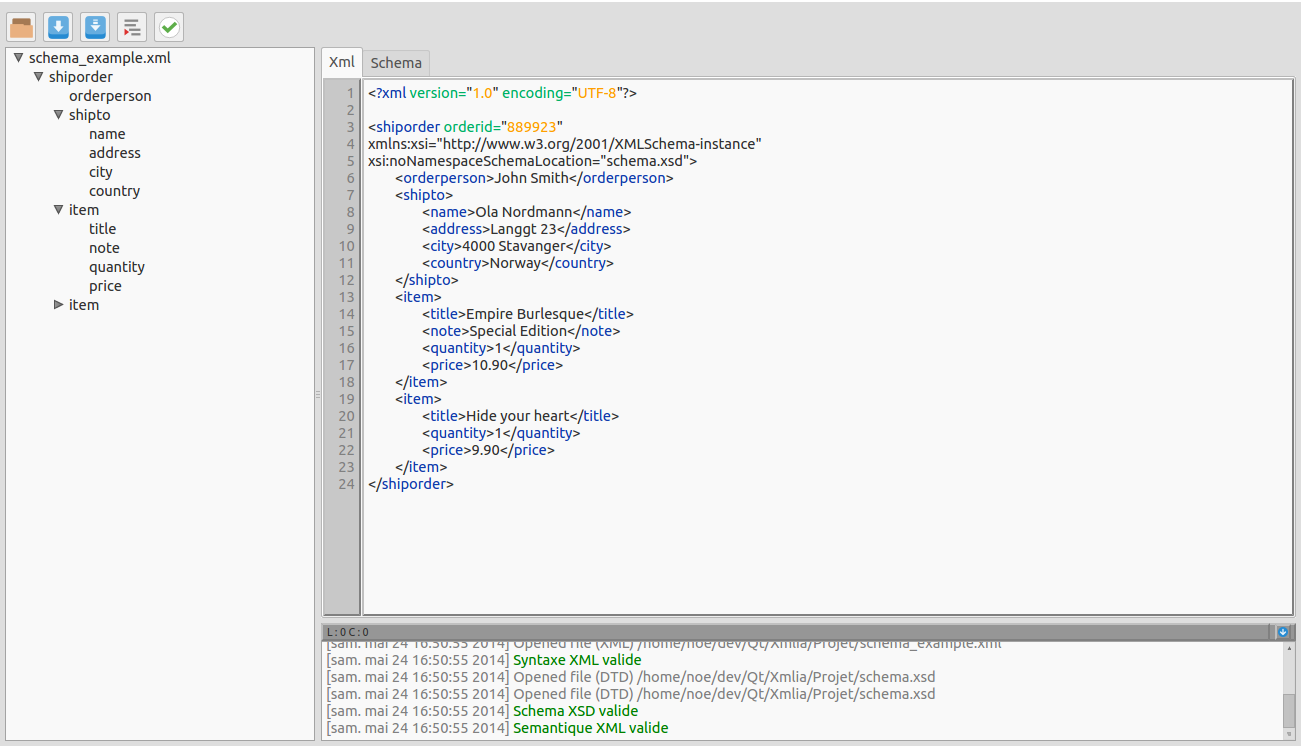
\includegraphics[scale=0.2]{images/final.png}
	\end{frame}


	\section{Conclusion}

	\begin{frame}
		\frametitle{Conclusion}
		\begin{itemize}
			\item Développement sous Qt
			\item Travail en groupe
			\item En bref
		\end{itemize}
	\end{frame}



\end{document}
